% Options for packages loaded elsewhere
\PassOptionsToPackage{unicode}{hyperref}
\PassOptionsToPackage{hyphens}{url}
%
\documentclass[
]{article}
\usepackage{lmodern}
\usepackage{amssymb,amsmath}
\usepackage{ifxetex,ifluatex}
\ifnum 0\ifxetex 1\fi\ifluatex 1\fi=0 % if pdftex
  \usepackage[T1]{fontenc}
  \usepackage[utf8]{inputenc}
  \usepackage{textcomp} % provide euro and other symbols
\else % if luatex or xetex
  \usepackage{unicode-math}
  \defaultfontfeatures{Scale=MatchLowercase}
  \defaultfontfeatures[\rmfamily]{Ligatures=TeX,Scale=1}
\fi
% Use upquote if available, for straight quotes in verbatim environments
\IfFileExists{upquote.sty}{\usepackage{upquote}}{}
\IfFileExists{microtype.sty}{% use microtype if available
  \usepackage[]{microtype}
  \UseMicrotypeSet[protrusion]{basicmath} % disable protrusion for tt fonts
}{}
\makeatletter
\@ifundefined{KOMAClassName}{% if non-KOMA class
  \IfFileExists{parskip.sty}{%
    \usepackage{parskip}
  }{% else
    \setlength{\parindent}{0pt}
    \setlength{\parskip}{6pt plus 2pt minus 1pt}}
}{% if KOMA class
  \KOMAoptions{parskip=half}}
\makeatother
\usepackage{xcolor}
\IfFileExists{xurl.sty}{\usepackage{xurl}}{} % add URL line breaks if available
\IfFileExists{bookmark.sty}{\usepackage{bookmark}}{\usepackage{hyperref}}
\hypersetup{
  pdftitle={Distance and dissimilarities},
  hidelinks,
  pdfcreator={LaTeX via pandoc}}
\urlstyle{same} % disable monospaced font for URLs
\usepackage[margin=1in]{geometry}
\usepackage{color}
\usepackage{fancyvrb}
\newcommand{\VerbBar}{|}
\newcommand{\VERB}{\Verb[commandchars=\\\{\}]}
\DefineVerbatimEnvironment{Highlighting}{Verbatim}{commandchars=\\\{\}}
% Add ',fontsize=\small' for more characters per line
\usepackage{framed}
\definecolor{shadecolor}{RGB}{248,248,248}
\newenvironment{Shaded}{\begin{snugshade}}{\end{snugshade}}
\newcommand{\AlertTok}[1]{\textcolor[rgb]{0.94,0.16,0.16}{#1}}
\newcommand{\AnnotationTok}[1]{\textcolor[rgb]{0.56,0.35,0.01}{\textbf{\textit{#1}}}}
\newcommand{\AttributeTok}[1]{\textcolor[rgb]{0.77,0.63,0.00}{#1}}
\newcommand{\BaseNTok}[1]{\textcolor[rgb]{0.00,0.00,0.81}{#1}}
\newcommand{\BuiltInTok}[1]{#1}
\newcommand{\CharTok}[1]{\textcolor[rgb]{0.31,0.60,0.02}{#1}}
\newcommand{\CommentTok}[1]{\textcolor[rgb]{0.56,0.35,0.01}{\textit{#1}}}
\newcommand{\CommentVarTok}[1]{\textcolor[rgb]{0.56,0.35,0.01}{\textbf{\textit{#1}}}}
\newcommand{\ConstantTok}[1]{\textcolor[rgb]{0.00,0.00,0.00}{#1}}
\newcommand{\ControlFlowTok}[1]{\textcolor[rgb]{0.13,0.29,0.53}{\textbf{#1}}}
\newcommand{\DataTypeTok}[1]{\textcolor[rgb]{0.13,0.29,0.53}{#1}}
\newcommand{\DecValTok}[1]{\textcolor[rgb]{0.00,0.00,0.81}{#1}}
\newcommand{\DocumentationTok}[1]{\textcolor[rgb]{0.56,0.35,0.01}{\textbf{\textit{#1}}}}
\newcommand{\ErrorTok}[1]{\textcolor[rgb]{0.64,0.00,0.00}{\textbf{#1}}}
\newcommand{\ExtensionTok}[1]{#1}
\newcommand{\FloatTok}[1]{\textcolor[rgb]{0.00,0.00,0.81}{#1}}
\newcommand{\FunctionTok}[1]{\textcolor[rgb]{0.00,0.00,0.00}{#1}}
\newcommand{\ImportTok}[1]{#1}
\newcommand{\InformationTok}[1]{\textcolor[rgb]{0.56,0.35,0.01}{\textbf{\textit{#1}}}}
\newcommand{\KeywordTok}[1]{\textcolor[rgb]{0.13,0.29,0.53}{\textbf{#1}}}
\newcommand{\NormalTok}[1]{#1}
\newcommand{\OperatorTok}[1]{\textcolor[rgb]{0.81,0.36,0.00}{\textbf{#1}}}
\newcommand{\OtherTok}[1]{\textcolor[rgb]{0.56,0.35,0.01}{#1}}
\newcommand{\PreprocessorTok}[1]{\textcolor[rgb]{0.56,0.35,0.01}{\textit{#1}}}
\newcommand{\RegionMarkerTok}[1]{#1}
\newcommand{\SpecialCharTok}[1]{\textcolor[rgb]{0.00,0.00,0.00}{#1}}
\newcommand{\SpecialStringTok}[1]{\textcolor[rgb]{0.31,0.60,0.02}{#1}}
\newcommand{\StringTok}[1]{\textcolor[rgb]{0.31,0.60,0.02}{#1}}
\newcommand{\VariableTok}[1]{\textcolor[rgb]{0.00,0.00,0.00}{#1}}
\newcommand{\VerbatimStringTok}[1]{\textcolor[rgb]{0.31,0.60,0.02}{#1}}
\newcommand{\WarningTok}[1]{\textcolor[rgb]{0.56,0.35,0.01}{\textbf{\textit{#1}}}}
\usepackage{longtable,booktabs}
% Correct order of tables after \paragraph or \subparagraph
\usepackage{etoolbox}
\makeatletter
\patchcmd\longtable{\par}{\if@noskipsec\mbox{}\fi\par}{}{}
\makeatother
% Allow footnotes in longtable head/foot
\IfFileExists{footnotehyper.sty}{\usepackage{footnotehyper}}{\usepackage{footnote}}
\makesavenoteenv{longtable}
\usepackage{graphicx,grffile}
\makeatletter
\def\maxwidth{\ifdim\Gin@nat@width>\linewidth\linewidth\else\Gin@nat@width\fi}
\def\maxheight{\ifdim\Gin@nat@height>\textheight\textheight\else\Gin@nat@height\fi}
\makeatother
% Scale images if necessary, so that they will not overflow the page
% margins by default, and it is still possible to overwrite the defaults
% using explicit options in \includegraphics[width, height, ...]{}
\setkeys{Gin}{width=\maxwidth,height=\maxheight,keepaspectratio}
% Set default figure placement to htbp
\makeatletter
\def\fps@figure{htbp}
\makeatother
\setlength{\emergencystretch}{3em} % prevent overfull lines
\providecommand{\tightlist}{%
  \setlength{\itemsep}{0pt}\setlength{\parskip}{0pt}}
\setcounter{secnumdepth}{-\maxdimen} % remove section numbering

\title{Distance and dissimilarities}
\author{}
\date{\vspace{-2.5em}}

\begin{document}
\maketitle

{
\setcounter{tocdepth}{2}
\tableofcontents
}
\begin{Shaded}
\begin{Highlighting}[]
\NormalTok{knitr}\OperatorTok{::}\NormalTok{opts_chunk}\OperatorTok{$}\KeywordTok{set}\NormalTok{(}\DataTypeTok{echo =} \OtherTok{TRUE}\NormalTok{)}
\CommentTok{#install.packages("dplyr")}
\CommentTok{#install.packages("stargazer")}
\CommentTok{#install.packages("ade4")}
\CommentTok{#install.packages("magrittr")}
\CommentTok{#install.packages("cluster")}
\end{Highlighting}
\end{Shaded}

\begin{Shaded}
\begin{Highlighting}[]
\NormalTok{x =}\StringTok{ }\KeywordTok{c}\NormalTok{(}\DecValTok{0}\NormalTok{, }\DecValTok{0}\NormalTok{)}
\NormalTok{y =}\StringTok{ }\KeywordTok{c}\NormalTok{(}\DecValTok{6}\NormalTok{,}\DecValTok{6}\NormalTok{)}
\KeywordTok{dist}\NormalTok{(}\KeywordTok{rbind}\NormalTok{(x, y), }\DataTypeTok{method =} \StringTok{"canberra"}\NormalTok{)}
\end{Highlighting}
\end{Shaded}

\begin{verbatim}
##   x
## y 2
\end{verbatim}

\begin{Shaded}
\begin{Highlighting}[]
\DecValTok{6}\OperatorTok{/}\DecValTok{6}\OperatorTok{+}\DecValTok{6}\OperatorTok{/}\DecValTok{6}
\end{Highlighting}
\end{Shaded}

\begin{verbatim}
## [1] 2
\end{verbatim}

\hypertarget{exercice-32}{%
\section{Exercice 32}\label{exercice-32}}

\begin{itemize}
\tightlist
\item
  Prove that the Canberra distance is a true distance.
\end{itemize}

\hypertarget{minkowski-distance}{%
\section{Minkowski distance}\label{minkowski-distance}}

\begin{itemize}
\tightlist
\item
  Both the Euclidian and the Manattan distances are special cases of the
  Minkowski distance which is defined, for \(p\geq 1\), by: \[
  d(\mathbf{x},\mathbf{y})=
  \left[\sum_{i=1} |x_i-y_i|^{p}\right]^{1/p}.
  \]
\item
  For \(p=1\), we get the Manhattan distance.
\item
  For \(p=2\), we get the Euclidian distance.
\item
  Let us also define:
  \[\|\mathbf{x}\|_p\equiv\left[\sum_{i=1}^n |x_i|^{p}\right]^{1/p},\]
  where \(\|\mathbf{\cdot}\|_p\) is known as the \(p\)-norm or Minkowski
  norm.
\item
  Note that the Minkowski distance and norm are related by:
\end{itemize}

\[d(\mathbf{x},\mathbf{y})=\|\mathbf{x}-\mathbf{y}\|_p.\]

\begin{itemize}
\tightlist
\item
  Conversely, we have:
\end{itemize}

\[\|\mathbf{x}\|_p=d(\mathbf{x},\mathbf{0}),\]

where \(\mathbf{0}\) is the null-vetor of \(\mathbb{R}^n\).

\begin{Shaded}
\begin{Highlighting}[]
\KeywordTok{library}\NormalTok{(}\StringTok{"ggplot2"}\NormalTok{)}
\NormalTok{x =}\StringTok{ }\KeywordTok{c}\NormalTok{(}\DecValTok{0}\NormalTok{, }\DecValTok{0}\NormalTok{)}
\NormalTok{y =}\StringTok{ }\KeywordTok{c}\NormalTok{(}\DecValTok{6}\NormalTok{,}\DecValTok{6}\NormalTok{)}
\NormalTok{MinkowDist=}\KeywordTok{c}\NormalTok{()}
\ControlFlowTok{for}\NormalTok{ (p }\ControlFlowTok{in} \KeywordTok{seq}\NormalTok{(}\DecValTok{1}\NormalTok{,}\DecValTok{30}\NormalTok{,.}\DecValTok{01}\NormalTok{))}
\NormalTok{\{}
\NormalTok{MinkowDist=}\KeywordTok{c}\NormalTok{(MinkowDist,}\KeywordTok{dist}\NormalTok{(}\KeywordTok{rbind}\NormalTok{(x, y), }\DataTypeTok{method =} \StringTok{"minkowski"}\NormalTok{, }\DataTypeTok{p =}\NormalTok{ p))     }
\NormalTok{\}}
\KeywordTok{ggplot}\NormalTok{(}\DataTypeTok{data =}\KeywordTok{data.frame}\NormalTok{(}\DataTypeTok{x =} \KeywordTok{seq}\NormalTok{(}\DecValTok{1}\NormalTok{,}\DecValTok{30}\NormalTok{,.}\DecValTok{01}\NormalTok{), }\DataTypeTok{y=}\NormalTok{MinkowDist ) , }\DataTypeTok{mapping =} \KeywordTok{aes}\NormalTok{(}\DataTypeTok{x =}\NormalTok{ x, }\DataTypeTok{y =}\NormalTok{ y))}\OperatorTok{+}\KeywordTok{geom_point}\NormalTok{(}\DataTypeTok{size=}\NormalTok{.}\DecValTok{1}\NormalTok{,}\DataTypeTok{color=}\StringTok{"red"}\NormalTok{)}\OperatorTok{+}\KeywordTok{xlim}\NormalTok{(}\DecValTok{1}\NormalTok{,}\DecValTok{11}\NormalTok{)}\OperatorTok{+}\KeywordTok{xlab}\NormalTok{(}\StringTok{"p"}\NormalTok{)}\OperatorTok{+}\KeywordTok{ylab}\NormalTok{(}\StringTok{"Minkowski Distance"}\NormalTok{)}\OperatorTok{+}\KeywordTok{ggtitle}\NormalTok{(}\StringTok{"Minkowski distance wrt p"}\NormalTok{)}
\end{Highlighting}
\end{Shaded}

\begin{verbatim}
## Warning: Removed 1900 rows containing missing values (geom_point).
\end{verbatim}

\includegraphics{Main2_files/figure-latex/unnamed-chunk-3-1.pdf}

\hypertarget{chebyshev-distance}{%
\section{Chebyshev distance}\label{chebyshev-distance}}

\begin{itemize}
\tightlist
\item
  At the limit, we get the Chebyshev distance which is defined by: \[
  d(\mathbf{x},\mathbf{y})=\max_{i=1,\cdots,n}(|x_i-y_i|)=\lim_{p\rightarrow\infty}
  \left[\sum_{i=1} |x_i-y_i|^{p}\right]^{1/p}.
  \]
\item
  The corresponding norm is: \[
  \|\mathbf{x}|_\infty=\max_{i=1,\cdots,n}(|x_i|).
  \]
\end{itemize}

\hypertarget{minkowski-inequality}{%
\section{Minkowski inequality}\label{minkowski-inequality}}

\begin{itemize}
\item
  The proof of the triangular inequality A3 is based on the Minkowski
  inequality:
\item
  For any nonnegative real numbers \(a_1,\cdots,a_n\);
  \(b_1,\cdots,b_n\), and for any \(p\geq 1\), we have: \[
  \left[\sum_{i=1}^n (a_i+b_i)^{p}\right]^{1/p}\leq
  \left[\sum_{i=1}^n a_i^{p}\right]^{1/p}
  +\left[\sum_{i=1}^n b_i^{p}\right]^{1/p}.
  \]
\item
  To prove that the Minkowski distance satisfies A3, notice that \[
   \sum_{i=1}^n|x_i-z_i|^{p}= \sum_{i=1}^n|(x_i-y_i)+(y_i-z_i)|^{p}.
  \]
\item
  Since for any reals \(x,y\), we have: \(|x+y|\leq |x|+|y|\), and using
  the fact that \(x^p\) is increasing in \(x\geq 0\), we obtain: \[
   \sum_{i=1}^n|x_i-z_i|^{p}\leq \sum_{i=1}^n(|x_i-y_i|+|y_i-z_i|)^{p}.
  \]
\item
  Applying the Minkowski inequality with \(a_i=|x_i-y_i|\) and
  \(b_i=|y_i-z_i|\), \(i=1,\cdots,n\), we get: \[
   \sum_{i=1}^n|x_i-z_i|^{p}\leq \left(\sum_{i=1}^n |x_i-y_i|^{p}\right)^{1/p}+\left(\sum_{i=1}^n |y_i-z_i|^{p}\right)^{1/p}.
  \]
\end{itemize}

\hypertarget{huxf6lder-inequality}{%
\section{Hölder inequality}\label{huxf6lder-inequality}}

\begin{itemize}
\tightlist
\item
  The proof of the Minkowski inequality itself requires the Hölder
  inequality:
\item
  For any nonnegative real numbers \(a_1,\cdots,a_n\);
  \(b_1,\cdots,b_n\), and any \(p,q>1\) with \(1/p+1/q=1\), we have: \[
  \sum_{i=1}^n a_ib_i\leq
  \left[\sum_{i=1}^n a_i^{p}\right]^{1/p}
  \left[\sum_{i=1}^n b_i^{q}\right]^{1/q}
  \]
\item
  The proof of the Hölder inequality relies on the Young inequality:
\item
  For any \(a,b>0\), we have \[
  ab\leq \frac{a^p}{p}+\frac{b^q}{q},
  \] with equality occuring iff: \(a^p=b^q\).
\item
  To prove the Young inequality, one can use the (strict) convexity of
  the exponential function.
\item
  For any reals \(x,y\), we have: \[
  e^{\frac{x}{p}+\frac{y}{q} }\leq \frac{e^{x}}{p}+\frac{e^{y}}{q}. 
  \]
\item
  We then set: \(x=p\ln a\) and \(y=q\ln b\) to get the Young
  inequality.
\item
  A good reference on inequalities is: Z. Cvetkovski, Inequalities:
  theorems, techniques and selected problems, 2012, Springer Science \&
  Business Media. \# Cauchy-Schwartz inequality
\item
  Note that the triangular inequality for the Minkowski distance
  implies: \[
  \sum_{i=1}^n |x_i|\leq
  \left[\sum_{i=1}^n |x_i|^{p}\right]^{1/p}.
  \]
\item
  Note that for \(p=2\), we have \(q=2\). The Hölder inequality implies
  for that special case \[
  \sum_{i=1}^n|x_iy_i|\leq\sqrt{\sum_{i=1}^n x_i^2}\sqrt{\sum_{i=1}^n y_i^2}. 
  \]
\item
  Since the LHS od thes above inequality is greater then
  \(|\sum_{i=1}^nx_iy_i|\), we get the Cauchy-Schwartz inequality
\end{itemize}

\[
|\sum_{i=1}^nx_iy_i|\leq\sqrt{\sum_{i=1}^n x_i^2}\sqrt{\sum_{i=1}^n y_i^2}. 
\] * Using the dot product notation called also scalar product noation:
\(\mathbf{x\cdot y}=\sum_{i=1}^nx_iy_i\), and the norm notation
\(\|\mathbf{\cdot}\|_2 \|\), the Cauchy-Schwart inequality is: \[
|\mathbf{x\cdot y} | \leq \|\mathbf{x}\|_2 \| \mathbf{y}\|_2.
\]

\hypertarget{pearson-correlation-distance}{%
\section{Pearson correlation
distance}\label{pearson-correlation-distance}}

\begin{itemize}
\item
  The Pearson correlation coefficient is a similarity measure on
  \(\mathbb{R}^n\) defined by: \[
  \rho(\mathbf{x},\mathbf{y})=
  \frac{\sum_{i=1}^n (x_i-\bar{\mathbf{x}})(y_i-\bar{\mathbf{y}})}{{\sqrt{\sum_{i=1}^n (x_i-\bar{\mathbf{x}})^2\sum_{i=1}^n (y_i-\bar{\mathbf{y}})^2}}},
  \] where \(\bar{\mathbf{x}}\) is the mean of the vector \(\mathbf{x}\)
  defined by: \[\bar{\mathbf{x}}=\frac{1}{n}\sum_{i=1}^n x_i,\]
\item
  Note that the Pearson correlation coefficient satisfies P2 and is
  invariant to any positive linear transformation, i.e.:
  \[\rho(\alpha\mathbf{x},\mathbf{y})=\rho(\mathbf{x},\mathbf{y}),\] for
  any \(\alpha>0\).
\item
  The Pearson distance (or correlation distance) is defined by: \[
  d(\mathbf{x},\mathbf{y})=1-\rho(\mathbf{x},\mathbf{y}).\]
\item
  Note that the Pearson distance does not satisfy A1 since
  \(d(\mathbf{x},\mathbf{x})=0\) for any non-zero vector \(\mathbf{x}\).
  It neither satisfies the triangle inequality. However, the symmetry
  property is fullfilled.
\end{itemize}

\hypertarget{cosine-correlation-distance}{%
\section{Cosine correlation
distance}\label{cosine-correlation-distance}}

\begin{itemize}
\tightlist
\item
  The cosine of the angle \(\theta\) between two vectors \(\mathbf{x}\)
  and \(\mathbf{y}\) is a measure of similarity given by: \[
  \cos(\theta)=\frac{\mathbf{x}\cdot \mathbf{y}}{\|\mathbf{x}\|_2\|\mathbf{y}\|_2}=\frac{\sum_{i=1}^n x_i y_i}{{\sqrt{\sum_{i=1}^n x_i^2\sum_{i=1}^n y_i^2}}}.
  \]
\item
  Note that the cosine of the angle between the two centred vectors
  \(\mathbf{x}-\bar{\mathbf{x}}\mathbf{1}\) and
  \(\mathbf{y}-\bar{\mathbf{y}}\mathbf{1}\) coincides with the Pearson
  correlation coefficient of \(\mathbf{x}\) and \(\mathbf{y}\), where
  \(\mathbf{1}\) is a vector of units of \(\mathbb{R}^n\).
\item
  The cosine correlation distance is defined by: \[
  d(\mathbf{x},\mathbf{y})=1-\cos(\theta).
  \]
\item
  It shares similar properties than the Pearson correlation distance.
  Likewise, Axioms A1 and A3 are not satisfied.
\end{itemize}

\hypertarget{spearman-correlation-distance}{%
\section{Spearman correlation
distance}\label{spearman-correlation-distance}}

\begin{itemize}
\tightlist
\item
  To calculate the Spearman's rank-order correlation, we need to map
  seperately each of the vectors to ranked data values:
  \[\mathbf{x}\rightarrow \text{rank}(\mathbf{x})=(x_1^r,\cdots,x_n^r).\]
\item
  Here, \(x_i^r\) is the rank of \(x_i\) among the set of values of
  \(\mathbf{x}\).
\item
  We illustrate this transformation with a simple example:
\item
  If \(\mathbf{x}=(3, 1, 4, 15, 92)\), then the rank-order vector is
  \(\text{rank}(\mathbf{x})=(2,1,3,4,5)\).
\end{itemize}

\begin{Shaded}
\begin{Highlighting}[]
\NormalTok{x=}\KeywordTok{c}\NormalTok{(}\DecValTok{3}\NormalTok{, }\DecValTok{1}\NormalTok{, }\DecValTok{4}\NormalTok{, }\DecValTok{15}\NormalTok{, }\DecValTok{92}\NormalTok{)}
\KeywordTok{rank}\NormalTok{(x)}
\end{Highlighting}
\end{Shaded}

\begin{verbatim}
## [1] 2 1 3 4 5
\end{verbatim}

\begin{itemize}
\tightlist
\item
  The Spearman's rank correlation of two numerical variables
  \(\mathbf{x}\) and \(\mathbf{y}\) is simply the Pearson correlation of
  the two correspnding rank-order variables \(\text{rank}(\mathbf{x})\)
  and \(\text{rank}(\mathbf{y})\),
  i.e.~\(\rho(\text{rank}(\mathbf{x}),\text{rank}(\mathbf{y}))\). This
  measure is is useful because it is more robust against outliers than
  the Pearson correlation.
\item
  If all the \(n\) ranks are distinct, it can be computed using the
  following formula: \[
  \rho(\text{rank}(\mathbf{x}),\text{rank}(\mathbf{y}))=1-\frac{6\sum_{i=1}^n d_i^2}{n(n^2-1)},
  \] where \(d_i=x_i^r-y_i^r,\:i=1,\cdots,n\).
\item
  The spearman distance is then defined by: \[
  d(\mathbf{x},\mathbf{y})=1-\rho(\text{rank}(\mathbf{x}),\text{rank}(\mathbf{y})).
  \]
\item
  It can be shown that easaly that it is not a proper distance.
\item
  If all the \(n\) ranks are distinct, we get: \[
  d(\mathbf{x},\mathbf{y})=\frac{6\sum_{i=1}^n d_i^2}{n(n^2-1)}.
  \]
\end{itemize}

\begin{Shaded}
\begin{Highlighting}[]
\NormalTok{x=}\KeywordTok{c}\NormalTok{(}\DecValTok{3}\NormalTok{, }\DecValTok{1}\NormalTok{, }\DecValTok{4}\NormalTok{, }\DecValTok{15}\NormalTok{, }\DecValTok{92}\NormalTok{)}
\KeywordTok{rank}\NormalTok{(x)}
\end{Highlighting}
\end{Shaded}

\begin{verbatim}
## [1] 2 1 3 4 5
\end{verbatim}

\begin{Shaded}
\begin{Highlighting}[]
\NormalTok{y=}\KeywordTok{c}\NormalTok{(}\DecValTok{30}\NormalTok{,}\DecValTok{2}\NormalTok{ , }\DecValTok{9}\NormalTok{, }\DecValTok{20}\NormalTok{, }\DecValTok{48}\NormalTok{)}
\KeywordTok{rank}\NormalTok{(y)}
\end{Highlighting}
\end{Shaded}

\begin{verbatim}
## [1] 4 1 2 3 5
\end{verbatim}

\begin{Shaded}
\begin{Highlighting}[]
\NormalTok{d=}\KeywordTok{rank}\NormalTok{(x)}\OperatorTok{-}\KeywordTok{rank}\NormalTok{(y)}
\NormalTok{d}
\end{Highlighting}
\end{Shaded}

\begin{verbatim}
## [1] -2  0  1  1  0
\end{verbatim}

\begin{Shaded}
\begin{Highlighting}[]
\KeywordTok{cor}\NormalTok{(}\KeywordTok{rank}\NormalTok{(x),}\KeywordTok{rank}\NormalTok{(y))}
\end{Highlighting}
\end{Shaded}

\begin{verbatim}
## [1] 0.7
\end{verbatim}

\begin{Shaded}
\begin{Highlighting}[]
\DecValTok{1-6}\OperatorTok{*}\KeywordTok{sum}\NormalTok{(d}\OperatorTok{^}\DecValTok{2}\NormalTok{)}\OperatorTok{/}\NormalTok{(}\DecValTok{5}\OperatorTok{*}\NormalTok{(}\DecValTok{5}\OperatorTok{^}\DecValTok{2-1}\NormalTok{))}
\end{Highlighting}
\end{Shaded}

\begin{verbatim}
## [1] 0.7
\end{verbatim}

\hypertarget{kendall-tau-distance}{%
\section{Kendall tau distance}\label{kendall-tau-distance}}

\begin{itemize}
\tightlist
\item
  The Kendall rank correlation coefficient is calculated from the number
  of correspondances between the rankings of \(\mathbf{x}\) and the
  rankings of \(\mathbf{y}\).
\item
  The number of pairs of observations among \(n\) observations or values
  is: \[{n \choose 2} =\frac{n(n-1)}{2}.\]
\item
  The pairs of observations \((x_{i},x_{j})\) and \((y_{i},y_{j})\) are
  said to be \emph{concordant} if:
  \[\text{sign}(x_j-x_i)=\text{sign}(y_j-y_i),\] and to be
  \emph{discordant} if: \[\text{sign}(x_j-x_i)=-\text{sign}(y_j-y_i),\]
  where \(\text{sign}(\cdot)\) returns \(1\) for positive numbers and
  \(-1\) negative numbers and \(0\) otherwise.
\item
  If \(x_i=x_j\) or \(y_i=y_j\) (or both), there is a tie.
\item
  The Kendall \(\tau\) coefficient is defined by (neglecting ties):
  \[\tau =\frac {1}{n(n-1)}\sum_{i=1}^{n}\sum_{j=1}^n\text{sign}(x_j-x_i)\text{sign}(y_j-y_i).\]
\item
  Let \(n_c\) (resp. \(n_d\)) be the number of concordant (resp.
  discordant) pairs, we have \[\tau =\frac {2(n_c-n_d)}{n(n-1)}.\]
\item
  The Kendall tau distance is then:
  \[d(\mathbf{x},\mathbf{y})=1-\tau. \]
\item
  Remark: the triangular inequality may fail in cases where there are
  ties.
\end{itemize}

\begin{Shaded}
\begin{Highlighting}[]
\NormalTok{x=}\KeywordTok{c}\NormalTok{(}\DecValTok{3}\NormalTok{, }\DecValTok{1}\NormalTok{, }\DecValTok{4}\NormalTok{, }\DecValTok{15}\NormalTok{, }\DecValTok{92}\NormalTok{)}
\NormalTok{y=}\KeywordTok{c}\NormalTok{(}\DecValTok{30}\NormalTok{,}\DecValTok{2}\NormalTok{ , }\DecValTok{9}\NormalTok{, }\DecValTok{20}\NormalTok{, }\DecValTok{48}\NormalTok{)}
\NormalTok{tau=}\DecValTok{0}
\ControlFlowTok{for}\NormalTok{ (i }\ControlFlowTok{in} \DecValTok{1}\OperatorTok{:}\DecValTok{5}\NormalTok{)}
\NormalTok{\{  }
\NormalTok{tau=tau}\OperatorTok{+}\KeywordTok{sign}\NormalTok{(x }\OperatorTok{-}\NormalTok{x[i])}\OperatorTok\KeywordTok{sign}\NormalTok{(y }\OperatorTok{-}\NormalTok{y[i])}
\NormalTok{\}}
\NormalTok{tau=tau}\OperatorTok{/}\NormalTok{(}\DecValTok{5}\OperatorTok{*}\DecValTok{4}\NormalTok{)}
\NormalTok{tau}
\end{Highlighting}
\end{Shaded}

\begin{verbatim}
##      [,1]
## [1,]  0.6
\end{verbatim}

\begin{Shaded}
\begin{Highlighting}[]
\KeywordTok{cor}\NormalTok{(x,y, }\DataTypeTok{method=}\StringTok{"kendall"}\NormalTok{)}
\end{Highlighting}
\end{Shaded}

\begin{verbatim}
## [1] 0.6
\end{verbatim}

\hypertarget{variables-standardization}{%
\section{Variables standardization}\label{variables-standardization}}

\begin{itemize}
\tightlist
\item
  Variables are often standardized before measuring dissimilarities.
\item
  Standardization converts the original variables into uniteless
  variables.
\item
  A well known method is the z-score transformation: \[
  \mathbf{x}\rightarrow (\frac{x_1-\bar{\mathbf{x}}}{s_\mathbf{x}},\cdots,\frac{x_n-\bar{\mathbf{x}}}{s_\mathbf{x}}),
  \] where \(s_\mathbf{x}\) is the sample standard deviation given by:
  \[
  s_\mathbf{x}=\frac{1}{n-1}\sum_{i=1}^n(x_i-\bar{\mathbf{x}})^2.
  \]
\item
  The transformed variable will have a mean of \(0\) and a variance of
  \(1\).
\item
  The result obtained with Pearson correlation measures and standardized
  Euclidean distances are comparable.
\item
  For other methods, see: Milligan, G. W., \& Cooper, M. C. (1988). A
  study of standardization of variables in cluster analysis.
  \emph{Journal of classification}, \emph{5}(2), 181-204.
\end{itemize}

\begin{Shaded}
\begin{Highlighting}[]
\NormalTok{x=}\KeywordTok{c}\NormalTok{(}\DecValTok{3}\NormalTok{, }\DecValTok{1}\NormalTok{, }\DecValTok{4}\NormalTok{, }\DecValTok{15}\NormalTok{, }\DecValTok{92}\NormalTok{)}
\NormalTok{y=}\KeywordTok{c}\NormalTok{(}\DecValTok{30}\NormalTok{,}\DecValTok{2}\NormalTok{ , }\DecValTok{9}\NormalTok{, }\DecValTok{20}\NormalTok{, }\DecValTok{48}\NormalTok{)}
\NormalTok{(x}\OperatorTok{-}\KeywordTok{mean}\NormalTok{(x))}\OperatorTok{/}\KeywordTok{sd}\NormalTok{(x)}
\end{Highlighting}
\end{Shaded}

\begin{verbatim}
## [1] -0.5134116 -0.5647527 -0.4877410 -0.2053646  1.7712699
\end{verbatim}

\begin{Shaded}
\begin{Highlighting}[]
\KeywordTok{scale}\NormalTok{(x)}
\end{Highlighting}
\end{Shaded}

\begin{verbatim}
##            [,1]
## [1,] -0.5134116
## [2,] -0.5647527
## [3,] -0.4877410
## [4,] -0.2053646
## [5,]  1.7712699
## attr(,"scaled:center")
## [1] 23
## attr(,"scaled:scale")
## [1] 38.9551
\end{verbatim}

\begin{Shaded}
\begin{Highlighting}[]
\NormalTok{(y}\OperatorTok{-}\KeywordTok{mean}\NormalTok{(y))}\OperatorTok{/}\KeywordTok{sd}\NormalTok{(y)}
\end{Highlighting}
\end{Shaded}

\begin{verbatim}
## [1]  0.45263128 -1.09293895 -0.70654639 -0.09935809  1.44621214
\end{verbatim}

\begin{Shaded}
\begin{Highlighting}[]
\KeywordTok{scale}\NormalTok{(y)}
\end{Highlighting}
\end{Shaded}

\begin{verbatim}
##             [,1]
## [1,]  0.45263128
## [2,] -1.09293895
## [3,] -0.70654639
## [4,] -0.09935809
## [5,]  1.44621214
## attr(,"scaled:center")
## [1] 21.8
## attr(,"scaled:scale")
## [1] 18.11629
\end{verbatim}

\hypertarget{similarity-measures-for-binary-data}{%
\section{Similarity measures for binary
data}\label{similarity-measures-for-binary-data}}

\begin{itemize}
\item
  A common simple situation occurs when all information is of the
  presence/absence of 2-level qualitative characters.
\item
  We assume there are \(n\) characters.
\item
  *The presence of the character is coded by \(1\) and the absence by 0.
\item
  We have have at our disposal two vectors.
\item
  \(\mathbf{x}\) is observed for a first individual (or object).
\item
  \(\mathbf{y}\) is observed for a second individual.
\item
  We can then calculate the following four statistics:

  \(a=\mathbf{x\cdot y}=\sum_{i=1}^nx_iy_i.\)

  \(b=\mathbf{x\cdot (1-y)}=\sum_{i=1}^nx_i(1-y_i).\)

  \(c=\mathbf{(1-x)\cdot y}=\sum_{i=1}^n(1-x_i)y_i.\)

  \(d=\mathbf{(1-x)\cdot (1-y)}=\sum_{i=1}^n(1-x_i)(1-y_i).\)
\item
  The counts of matches are \(a\) for \((1,1)\) and \(d\) for \((0,0)\);
\item
  The counts of mismatches are \(b\) for \((1,0)\) and \(c\) for
  \((0,1)\).
\item
  Note that obviously: \(a+b+c+d= n\).
\item
  This gives a very useful \(2 \times 2\) association table.
\end{itemize}

\begin{longtable}[]{@{}llccc@{}}
\toprule
& & Second individual & &\tabularnewline
\midrule
\endhead
& & 1 & 0 & \emph{Totals}\tabularnewline
\textbf{First individual} & 1 & \(a\) & \(b\) & \(a+b\)\tabularnewline
& 0 & \(c\) & \(d\) & \(c+d\)\tabularnewline
\emph{Totals} & & \(a+c\) & \(b+d\) & \(n\)\tabularnewline
\bottomrule
\end{longtable}

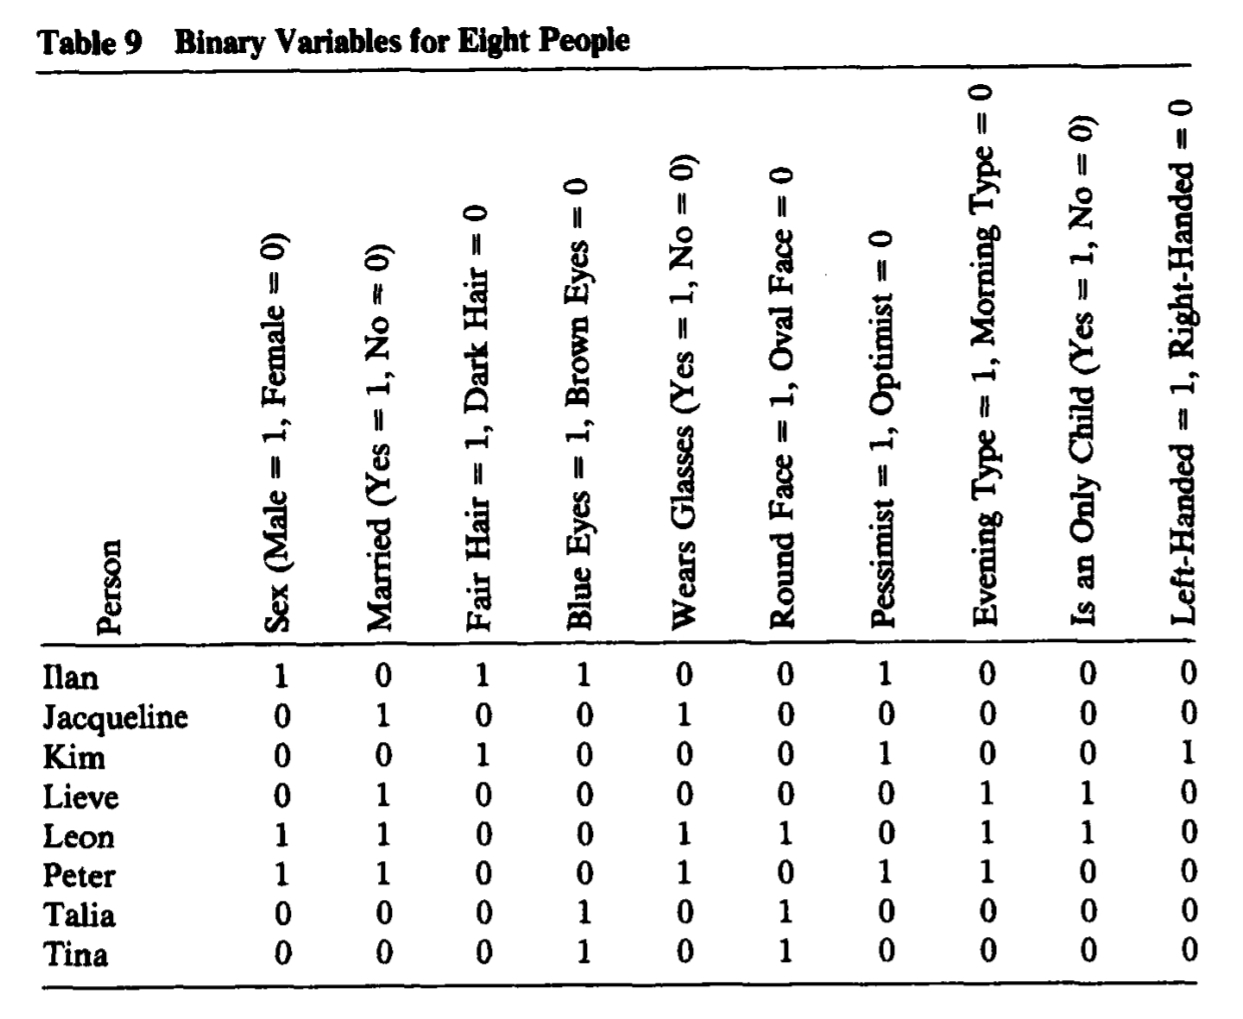
\includegraphics{https://raw.githubusercontent.com/karkil2205/Usid13Chapter1/master/KAUFMANBinarydata.jpg}
\emph{Table from Kaufman, L., \& Rousseeuw, P. J. (2009). \emph{Finding
groups in data: an introduction to cluster analysis} (Vol. 344). John
Wiley \& Sons} * The data shows \(8\) people (individuals) and \(10\)
binary variables: * Sex, Married, Fair Hair, Blue Eyes, Wears Glasses,
Round Face, Pessimist, Evening Type, Is an Only Child, Left-Handed.

\begin{Shaded}
\begin{Highlighting}[]
\NormalTok{data=}\KeywordTok{c}\NormalTok{(}
\DecValTok{1}\NormalTok{,}\DecValTok{0}\NormalTok{,}\DecValTok{1}\NormalTok{,}\DecValTok{1}\NormalTok{,}\DecValTok{0}\NormalTok{,}\DecValTok{0}\NormalTok{,}\DecValTok{1}\NormalTok{,}\DecValTok{0}\NormalTok{,}\DecValTok{0}\NormalTok{,}\DecValTok{0}\NormalTok{,}
\DecValTok{0}\NormalTok{,}\DecValTok{1}\NormalTok{,}\DecValTok{0}\NormalTok{,}\DecValTok{0}\NormalTok{,}\DecValTok{1}\NormalTok{,}\DecValTok{0}\NormalTok{,}\DecValTok{0}\NormalTok{,}\DecValTok{0}\NormalTok{,}\DecValTok{0}\NormalTok{,}\DecValTok{0}\NormalTok{,}
\DecValTok{0}\NormalTok{,}\DecValTok{0}\NormalTok{,}\DecValTok{1}\NormalTok{,}\DecValTok{0}\NormalTok{,}\DecValTok{0}\NormalTok{,}\DecValTok{0}\NormalTok{,}\DecValTok{1}\NormalTok{,}\DecValTok{0}\NormalTok{,}\DecValTok{0}\NormalTok{,}\DecValTok{1}\NormalTok{,}
\DecValTok{0}\NormalTok{,}\DecValTok{1}\NormalTok{,}\DecValTok{0}\NormalTok{,}\DecValTok{0}\NormalTok{,}\DecValTok{0}\NormalTok{,}\DecValTok{0}\NormalTok{,}\DecValTok{0}\NormalTok{,}\DecValTok{1}\NormalTok{,}\DecValTok{1}\NormalTok{,}\DecValTok{0}\NormalTok{,}
\DecValTok{1}\NormalTok{,}\DecValTok{1}\NormalTok{,}\DecValTok{0}\NormalTok{,}\DecValTok{0}\NormalTok{,}\DecValTok{1}\NormalTok{,}\DecValTok{1}\NormalTok{,}\DecValTok{0}\NormalTok{,}\DecValTok{1}\NormalTok{,}\DecValTok{1}\NormalTok{,}\DecValTok{0}\NormalTok{,}
\DecValTok{1}\NormalTok{,}\DecValTok{1}\NormalTok{,}\DecValTok{0}\NormalTok{,}\DecValTok{0}\NormalTok{,}\DecValTok{1}\NormalTok{,}\DecValTok{0}\NormalTok{,}\DecValTok{1}\NormalTok{,}\DecValTok{1}\NormalTok{,}\DecValTok{0}\NormalTok{,}\DecValTok{0}\NormalTok{,}
\DecValTok{0}\NormalTok{,}\DecValTok{0}\NormalTok{,}\DecValTok{0}\NormalTok{,}\DecValTok{1}\NormalTok{,}\DecValTok{0}\NormalTok{,}\DecValTok{1}\NormalTok{,}\DecValTok{0}\NormalTok{,}\DecValTok{0}\NormalTok{,}\DecValTok{0}\NormalTok{,}\DecValTok{0}\NormalTok{,}
\DecValTok{0}\NormalTok{,}\DecValTok{0}\NormalTok{,}\DecValTok{0}\NormalTok{,}\DecValTok{1}\NormalTok{,}\DecValTok{0}\NormalTok{,}\DecValTok{1}\NormalTok{,}\DecValTok{0}\NormalTok{,}\DecValTok{0}\NormalTok{,}\DecValTok{0}\NormalTok{,}\DecValTok{0}
\NormalTok{)}
\NormalTok{data=}\KeywordTok{data.frame}\NormalTok{(}\KeywordTok{matrix}\NormalTok{(data, }\DataTypeTok{nrow=}\DecValTok{8}\NormalTok{,}\DataTypeTok{byrow=}\NormalTok{T))}
\KeywordTok{row.names}\NormalTok{(data)=}\KeywordTok{c}\NormalTok{(}\StringTok{"Ilan"}\NormalTok{,}\StringTok{"Jacqueline"}\NormalTok{,}\StringTok{"Kim"}\NormalTok{,}\StringTok{"Lieve"}\NormalTok{,}\StringTok{"Leon"}\NormalTok{,}\StringTok{"Peter"}\NormalTok{,}\StringTok{"Talia"}\NormalTok{,}\StringTok{"Tina"}\NormalTok{)}
\KeywordTok{names}\NormalTok{(data)=}\KeywordTok{c}\NormalTok{(}\StringTok{"Sex"}\NormalTok{, }\StringTok{"Married"}\NormalTok{, }\StringTok{"Fair Hair"}\NormalTok{, }\StringTok{"Blue Eyes"}\NormalTok{, }\StringTok{"Wears Glasses"}\NormalTok{, }\StringTok{"Round Face"}\NormalTok{, }\StringTok{"Pessimist"}\NormalTok{, }\StringTok{"Evening Type"}\NormalTok{, }\StringTok{"Is an Only Child"}\NormalTok{, }\StringTok{"Left-Handed"}\NormalTok{)}
\end{Highlighting}
\end{Shaded}

\begin{itemize}
\tightlist
\item
  We are comparing the records for Ilan with Talia.
\end{itemize}

\begin{Shaded}
\begin{Highlighting}[]
\NormalTok{x=data[}\StringTok{"Ilan"}\NormalTok{,]}
\NormalTok{y=data[}\StringTok{"Talia"}\NormalTok{,]}
\NormalTok{knitr}\OperatorTok{::}\KeywordTok{kable}\NormalTok{(}\KeywordTok{table}\NormalTok{(x, y)[}\DecValTok{2}\OperatorTok{:}\DecValTok{1}\NormalTok{,}\DecValTok{2}\OperatorTok{:}\DecValTok{1}\NormalTok{],}\StringTok{"pipe"}\NormalTok{)}
\end{Highlighting}
\end{Shaded}

\begin{longtable}[]{@{}lrr@{}}
\toprule
& 1 & 0\tabularnewline
\midrule
\endhead
1 & 1 & 3\tabularnewline
0 & 1 & 5\tabularnewline
\bottomrule
\end{longtable}

\begin{itemize}
\tightlist
\item
  Therefore: \(a = 1,\:b = 3,\: c = 1,\: d = 5\).
\item
  Note that interchanging Ilan and Talia would permute \(b\) and \(c\)
  while leaving \(a\) and \(d\) unchanged.
\item
  A good similarity or dissimilarity coefficient must treat \(b\) and
  \(c\) symmetrically.
\item
  A similarity measure is denoted by: \(s(\mathbf{x},\mathbf{y})\).
\item
  The corresponding distance is then defined as:
  \[d(\mathbf{x},\mathbf{y})=1-s(\mathbf{x},\mathbf{y}).\]
\item
  Alternatively, we have:
  \[d(\mathbf{x},\mathbf{y})=\sqrt{1-s(\mathbf{x},\mathbf{y})}.\]
\item
  A list of some of the similarity measures \(s(\mathbf{x},\mathbf{y})\)
  that have been suggested for binary data is shown below.
\item
  A more extensive list can be found in: Gower, J. C., \& Legendre, P.
  (1986). Metric and Euclidean properties of dissimilarity coefficients.
  \emph{Journal of classification}, \emph{3}(1), 5-48.
\end{itemize}

\begin{longtable}[]{@{}lcc@{}}
\toprule
\begin{minipage}[b]{0.26\columnwidth}\raggedright
Coefficient\strut
\end{minipage} & \begin{minipage}[b]{0.33\columnwidth}\centering
\(s(\mathbf{x},\mathbf{y})\)\strut
\end{minipage} & \begin{minipage}[b]{0.33\columnwidth}\centering
\(d(\mathbf{x},\mathbf{y})=1-s(\mathbf{x},\mathbf{y})\)\strut
\end{minipage}\tabularnewline
\midrule
\endhead
\begin{minipage}[t]{0.26\columnwidth}\raggedright
Simple matching\strut
\end{minipage} & \begin{minipage}[t]{0.33\columnwidth}\centering
\(\frac{a+d}{a+b+c+d}\)\strut
\end{minipage} & \begin{minipage}[t]{0.33\columnwidth}\centering
\(\frac{b+c}{a+b+c+d}\)\strut
\end{minipage}\tabularnewline
\begin{minipage}[t]{0.26\columnwidth}\raggedright
Jaccard\strut
\end{minipage} & \begin{minipage}[t]{0.33\columnwidth}\centering
\(\frac{a}{a+b+c}\)\strut
\end{minipage} & \begin{minipage}[t]{0.33\columnwidth}\centering
\(\frac{b+c}{a+b+c}\)\strut
\end{minipage}\tabularnewline
\begin{minipage}[t]{0.26\columnwidth}\raggedright
Rogers and Tanimoto (1960)\strut
\end{minipage} & \begin{minipage}[t]{0.33\columnwidth}\centering
\(\frac{a+d}{a+2(b+c)+d}\)\strut
\end{minipage} & \begin{minipage}[t]{0.33\columnwidth}\centering
\(\frac{2(b+c)}{a+2(b+c)+d}\)\strut
\end{minipage}\tabularnewline
\begin{minipage}[t]{0.26\columnwidth}\raggedright
Gower and Legendre (1986)\strut
\end{minipage} & \begin{minipage}[t]{0.33\columnwidth}\centering
\(\frac{2(a+d)}{2(a+d)+b+c}\)\strut
\end{minipage} & \begin{minipage}[t]{0.33\columnwidth}\centering
\(\frac{b+c}{2(a+d)+b+c}]\)\strut
\end{minipage}\tabularnewline
\begin{minipage}[t]{0.26\columnwidth}\raggedright
Gower and Legendre (1986)\strut
\end{minipage} & \begin{minipage}[t]{0.33\columnwidth}\centering
\(\frac{2a}{2a+b+c}\)\strut
\end{minipage} & \begin{minipage}[t]{0.33\columnwidth}\centering
\(\frac{b+c}{2a+b+c}\)\strut
\end{minipage}\tabularnewline
\bottomrule
\end{longtable}

\begin{itemize}
\item
  To calculate these coefficients, we use the function:
  \href{https://www.rdocumentation.org/packages/ade4/versions/1.7-16/topics/dist.binary}{dist.binary().}
\item
  All the distances in this package are of type
  \(d(\mathbf{x}.\mathbf{y})= \sqrt{1 - s(\mathbf{x}.\mathbf{y})}\).
\end{itemize}

\begin{Shaded}
\begin{Highlighting}[]
\KeywordTok{library}\NormalTok{(ade4)}
\NormalTok{a=}\DecValTok{1}
\NormalTok{b=}\DecValTok{3}
\NormalTok{c=}\DecValTok{1}
\NormalTok{d=}\DecValTok{5}
\KeywordTok{dist.binary}\NormalTok{(data[}\KeywordTok{c}\NormalTok{(}\StringTok{"Ilan"}\NormalTok{,}\StringTok{"Talia"}\NormalTok{),],}\DataTypeTok{method=}\DecValTok{2}\NormalTok{)}\OperatorTok{^}\DecValTok{2}
\end{Highlighting}
\end{Shaded}

\begin{verbatim}
  Ilan
\end{verbatim}

Talia 0.4

\begin{Shaded}
\begin{Highlighting}[]
\DecValTok{1}\OperatorTok{-}\NormalTok{(a}\OperatorTok{+}\NormalTok{d )}\OperatorTok{/}\NormalTok{(a}\OperatorTok{+}\NormalTok{b}\OperatorTok{+}\NormalTok{c}\OperatorTok{+}\NormalTok{d)}
\end{Highlighting}
\end{Shaded}

{[}1{]} 0.4

\begin{Shaded}
\begin{Highlighting}[]
\KeywordTok{dist.binary}\NormalTok{(data[}\KeywordTok{c}\NormalTok{(}\StringTok{"Ilan"}\NormalTok{,}\StringTok{"Talia"}\NormalTok{),],}\DataTypeTok{method=}\DecValTok{1}\NormalTok{)}\OperatorTok{^}\DecValTok{2}
\end{Highlighting}
\end{Shaded}

\begin{verbatim}
  Ilan
\end{verbatim}

Talia 0.8

\begin{Shaded}
\begin{Highlighting}[]
\DecValTok{1}\OperatorTok{-}\NormalTok{a}\OperatorTok{/}\NormalTok{(a}\OperatorTok{+}\NormalTok{b}\OperatorTok{+}\NormalTok{c)}
\end{Highlighting}
\end{Shaded}

{[}1{]} 0.8

\begin{Shaded}
\begin{Highlighting}[]
\KeywordTok{dist.binary}\NormalTok{(data[}\KeywordTok{c}\NormalTok{(}\StringTok{"Ilan"}\NormalTok{,}\StringTok{"Talia"}\NormalTok{),],}\DataTypeTok{method=}\DecValTok{4}\NormalTok{)}\OperatorTok{^}\DecValTok{2}
\end{Highlighting}
\end{Shaded}

\begin{verbatim}
       Ilan
\end{verbatim}

Talia 0.5714286

\begin{Shaded}
\begin{Highlighting}[]
\DecValTok{1}\OperatorTok{-}\NormalTok{(a}\OperatorTok{+}\NormalTok{d )}\OperatorTok{/}\NormalTok{(a}\OperatorTok{+}\DecValTok{2}\OperatorTok{*}\NormalTok{(b}\OperatorTok{+}\NormalTok{c)}\OperatorTok{+}\NormalTok{d)}
\end{Highlighting}
\end{Shaded}

{[}1{]} 0.5714286

\begin{Shaded}
\begin{Highlighting}[]
\CommentTok{# One Gower coefficient is missing}
\KeywordTok{dist.binary}\NormalTok{(data[}\KeywordTok{c}\NormalTok{(}\StringTok{"Ilan"}\NormalTok{,}\StringTok{"Talia"}\NormalTok{),],}\DataTypeTok{method=}\DecValTok{5}\NormalTok{)}\OperatorTok{^}\DecValTok{2}
\end{Highlighting}
\end{Shaded}

\begin{verbatim}
       Ilan
\end{verbatim}

Talia 0.6666667

\begin{Shaded}
\begin{Highlighting}[]
\DecValTok{1-2}\OperatorTok{*}\NormalTok{a}\OperatorTok{/}\NormalTok{(}\DecValTok{2}\OperatorTok{*}\NormalTok{a}\OperatorTok{+}\NormalTok{b}\OperatorTok{+}\NormalTok{c)}
\end{Highlighting}
\end{Shaded}

{[}1{]} 0.6666667 * The reason for such a large number of possible
measures has to do with the apparent uncertainty as to how to deal with
the count of zero-zero matches \(d\). * The measues embedding \(d\) are
sometimes called symmetrical. * The other measues are called
assymmetrical. * In some cases, of course, zero\_zero matches are
completely equivalent to one--one matches, and therefore should be
included in the calculated similarity measure. * An example is gender,
where there is no preference as to which of the two categories should be
coded zero or one. * But in other cases the inclusion or otherwise of
\(d\) is more problematic; for example, when the zero category
corresponds to the genuine absence of some property, such as wings in a
study of insects. \# Exercice 4 * Prove that the distances based on the
SimplemMatching coefficient and the Jaccard coefficient satisfy A3. *
Prove that the distances proposed by Gower and Legendre (1986) do not
satisfy A3. * Hint: Proofs and counterexamples have to be adapted from
in the paper: *
\href{https://drive.google.com/file/d/1PUQ7g9HIwwUG0CXbCsLA03hnApWMhjka/view?usp=drivesdk}{Gower,
J. C., \& Legendre, P. (1986). Metric and Euclidean properties of
dissimilarity coefficients. \emph{Journal of classification},
\emph{3}(1), 5-48.}

\hypertarget{nominal-variables}{%
\section{Nominal variables}\label{nominal-variables}}

\begin{itemize}
\item
  We previuosly studied above binary variables which can only take on
  two states coded as \(0,1\).
\item
  We generalize this approach to nominal variables which may take on
  more than two states.
\item
  Eye's color may have for example four states: blue, brown, green, grey
  .
\item
  Le \(M\) be the number of states and code the outcomes as
  \(1, \cdots, M\).
\item
  We could choose \(1 =\text{blue},\) \(2 =\text{brown},\)
  \(3 =\text{green},\) and \(4 =\text{grey}\).
\item
  These states are not ordered in any way
\item
  One strategy would be creating a new binary variable for each of the
  \(M\) nominal states.
\item
  Then to put it equal to \(1\) if the corresponding state occurs and to
  \(0\) otherwise.
\item
  After that, one could resort to one of the dissimilarity coeffi-
  cients of the previous subsection.
\item
  The most common way of measuring the similarity or dissimilarity
  between two objects through categorial variables is the simple
  matching approach.
\item
  If \(\mathbf{x},\mathbf{y},\) are both \(n\) nominal records for two
  individuals,
\item
  Let define the function: \[\delta(x_i,y_i)\equiv \begin{cases}0,
  \text{ if } x_i=y_i;\\1,\text{ if } x_i \neq y_i.\end{cases}\]
\item
  Let \(N_{a+d}\) be the number of attributes of the two individuals on
  which the two records match: \[N_{a+d}=\sum_{i=1}^n\delta(x_i,y_i).\]
\item
  Let \(N_{b+c}\) be the number of attributes on which the two records
  do not match: \[N_{b+c}= n - N_{a+d}.\]
\item
  Let \(N_d\) be the number of attributes on which the two records match
  in a ``not applicable'' category:
  \[N_{d}=\sum_{i=1}^n\delta(x_i,y_i).\]
\item
  The distance corresponding to the simple matching approach is: \[
  d(\mathbf{x},\mathbf{y})=\frac{\sum_{i=1}^n\delta(x_i,y_i)}{n}.
  \]
\item
  Therefore:
  \[d(\mathbf{x},\mathbf{y})=\frac{N_{a+d}}{N_{a+d}+N_{b+c}}.\]
\item
  Note that simple matching has exactly the same meaning as in the
  preceding section.
\end{itemize}

\hypertarget{gowers-dissimilarity}{%
\section{Gower's dissimilarity}\label{gowers-dissimilarity}}

\begin{itemize}
\tightlist
\item
  Gower's coefficient is a dissimilarity measure specifically designed
  for handling mixed attribute types or variables.
\item
  See: GOWER, John C. A general coefficient of similarity and some of
  its properties. \emph{Biometrics}, 1971, p.~857-871.
\item
  The coefficient is calculated as the weighted average of attribute
  contributions.
\item
  Weights usually used only to indicate which attribute values could
  actually be compared meaningfully.
\item
  The formula is: \[
  d(\mathbf{x},\mathbf{y})=\frac{\sum_{i=1}^n w_i \delta(x_i,y_i)}{\sum_{i=1}^n w_i}.
  \]
\item
  The wheight \(w_i\) is put equal to \(1\) when both measurements
  \(x_i\) and \(y_i\) are nonmissing,
\item
  The number \(\delta(x_i,y_i)\) is the contribution of the \(i\)th
  measure or variable to the dissimilarity measure.
\item
  It the \(i\)th measure is nominal, we take\\
  \[
  \delta(x_i,y_i)\equiv \begin{cases}0,
  \text{ if } x_i=y_i;\\1,\text{ if } x_i \neq y_i.\end{cases}
  \]
\item
  If the \(i\)th measure is interval-scaled, we take instead: \[
  \delta(x_i,y_i)\equiv \frac{|x_i-y_i|}{R_i},
  \] where \(R_i\) is the range of variable \(i\) over the available
  data.
\item
  Consider the following data set:
\end{itemize}

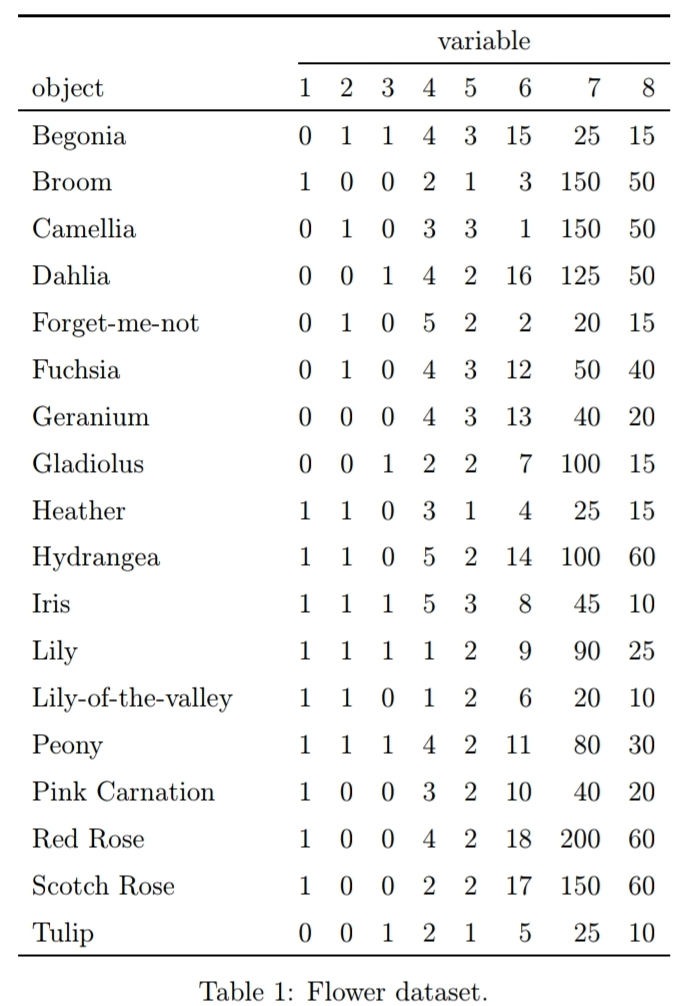
\includegraphics{https://raw.githubusercontent.com/karkil2205/Usid13Chapter1/master/flowers.jpg}
\emph{Data from: Struyf, A., Hubert, M., \& Rousseeuw, P. (1997).
Clustering in an object-oriented environment. \emph{Journal of
Statistical Software}, \emph{1}(4), 1-30.}

\begin{itemize}
\tightlist
\item
  The dataset contains 18 flowers and 8 characteristics:
\end{itemize}

\begin{enumerate}
\def\labelenumi{\arabic{enumi}.}
\tightlist
\item
  Winters: binary, indicates whether the plant may be left in the garden
  when it freezes.
\item
  Shadow: binary, shows whether the plant needs to stand in the shadow.
\item
  Tubers (Tubercule): asymmetric binary, distinguishes between plants
  with tubers and plants that grow in any other way.
\item
  Color: nominal, specifies the flower's color (1=white, 2=yellow, 3=
  pink, 4=red, 5= blue).
\item
  Soil: ordinal, indicates whether the plant grows in dry (1), normal
  (2), or wet (3) soil.
\item
  Preference: ordinal, someone's preference ranking, going from 1 to 18.
\item
  Height: interval scaled, the plant's height in centimeters.
\item
  Distance: interval scaled, the distance in centimeters that should be
  left between the plants.
\end{enumerate}

\begin{itemize}
\tightlist
\item
  The dissimilarity between Begonia and Broom (Genêt) can be calculated
  as follows:
  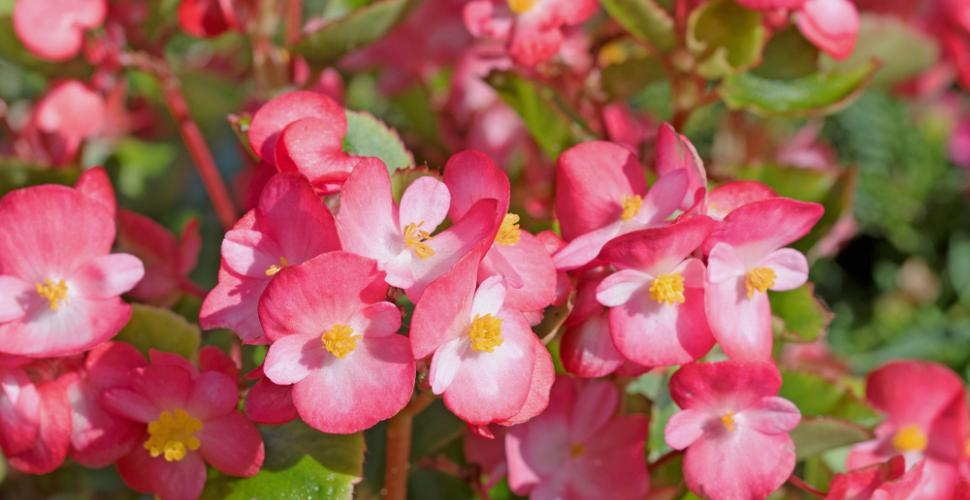
\includegraphics{https://raw.githubusercontent.com/karkil2205/Usid13Chapter1/master/Begonia.jpg}
  \emph{Begonia}
  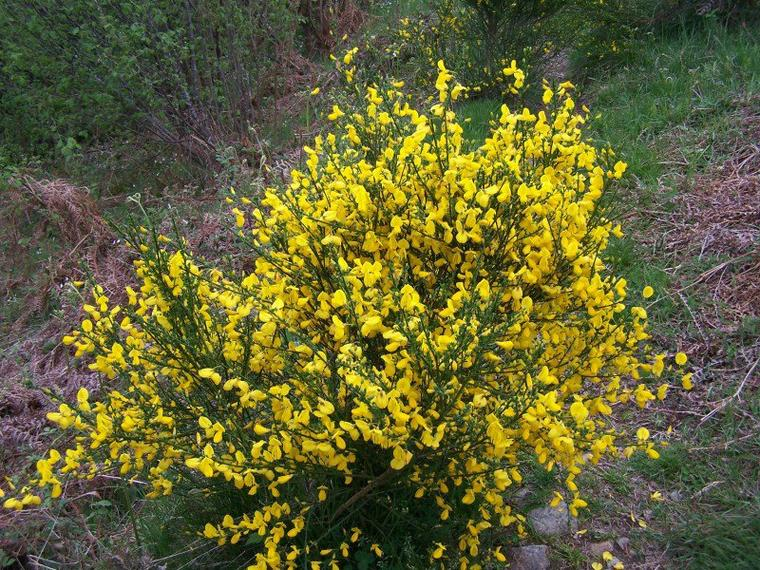
\includegraphics{https://raw.githubusercontent.com/karkil2205/Usid13Chapter1/master/Genet.jpeg}
  \emph{Genêt}
\end{itemize}

\begin{Shaded}
\begin{Highlighting}[]
\KeywordTok{library}\NormalTok{(cluster)}
\KeywordTok{library}\NormalTok{(dplyr)}
\end{Highlighting}
\end{Shaded}

\begin{verbatim}
## 
## Attaching package: 'dplyr'
\end{verbatim}

\begin{verbatim}
## The following objects are masked from 'package:stats':
## 
##     filter, lag
\end{verbatim}

\begin{verbatim}
## The following objects are masked from 'package:base':
## 
##     intersect, setdiff, setequal, union
\end{verbatim}

\begin{Shaded}
\begin{Highlighting}[]
\NormalTok{data <-flower }\OperatorTok\StringTok{ }
\KeywordTok{rename}\NormalTok{(}\DataTypeTok{Winters=}\NormalTok{V1,}\DataTypeTok{Shadow=}\NormalTok{V2,}\DataTypeTok{Tubers=}\NormalTok{V3,}\DataTypeTok{Color=}\NormalTok{V4,}\DataTypeTok{Soil=}\NormalTok{V5,}\DataTypeTok{Preference=}\NormalTok{V6,}\DataTypeTok{Height=}\NormalTok{V7,}\DataTypeTok{Distance=}\NormalTok{V8) }\OperatorTok
\KeywordTok{mutate}\NormalTok{(}\DataTypeTok{Winters=}\KeywordTok{recode}\NormalTok{(Winters,}\StringTok{"1"}\NormalTok{=}\StringTok{"Yes"}\NormalTok{,}\StringTok{"0"}\NormalTok{=}\StringTok{"No"}\NormalTok{),}
      \DataTypeTok{Shadow=}\KeywordTok{recode}\NormalTok{(Shadow,}\StringTok{"1"}\NormalTok{=}\StringTok{"Yes"}\NormalTok{,}\StringTok{"0"}\NormalTok{=}\StringTok{"No"}\NormalTok{),}
      \DataTypeTok{Tubers=}\KeywordTok{recode}\NormalTok{(Tubers,}\StringTok{"1"}\NormalTok{=}\StringTok{"Yes"}\NormalTok{,}\StringTok{"0"}\NormalTok{=}\StringTok{"No"}\NormalTok{),}
      \DataTypeTok{Color=}\KeywordTok{recode}\NormalTok{(Color,}\StringTok{"1"}\NormalTok{=}\StringTok{"white"}\NormalTok{, }\StringTok{"2"}\NormalTok{=}\StringTok{"yellow"}\NormalTok{, }\StringTok{"3"}\NormalTok{=}\StringTok{ "pink"}\NormalTok{, }\StringTok{"4"}\NormalTok{=}\StringTok{"red"}\NormalTok{, }\StringTok{"5"}\NormalTok{=}\StringTok{"blue"}\NormalTok{),}
      \DataTypeTok{Soil=}\KeywordTok{recode}\NormalTok{(Soil,}\StringTok{"1"}\NormalTok{=}\StringTok{"dry"}\NormalTok{, }\StringTok{"2"}\NormalTok{=}\StringTok{"normal"}\NormalTok{, }\StringTok{"3"}\NormalTok{=}\StringTok{ "wet"}\NormalTok{)}
\NormalTok{      ) }
\end{Highlighting}
\end{Shaded}

\begin{Shaded}
\begin{Highlighting}[]
\NormalTok{res=}\KeywordTok{lapply}\NormalTok{(data,class)  }
\NormalTok{res=}\KeywordTok{as.data.frame}\NormalTok{(res)}
\NormalTok{res[}\DecValTok{1}\NormalTok{,] }\OperatorTok\StringTok{ }
\NormalTok{knitr}\OperatorTok{::}\KeywordTok{kable}\NormalTok{()}
\end{Highlighting}
\end{Shaded}

\begin{longtable}[]{@{}llllllll@{}}
\toprule
Winters & Shadow & Tubers & Color & Soil & Preference & Height &
Distance\tabularnewline
\midrule
\endhead
factor & factor & factor & factor & ordered & ordered & numeric &
numeric\tabularnewline
\bottomrule
\end{longtable}

\begin{Shaded}
\begin{Highlighting}[]
\NormalTok{flower[}\DecValTok{1}\OperatorTok{:}\DecValTok{2}\NormalTok{,]}
\end{Highlighting}
\end{Shaded}

\begin{verbatim}
##   V1 V2 V3 V4 V5 V6  V7 V8
## 1  0  1  1  4  3 15  25 15
## 2  1  0  0  2  1  3 150 50
\end{verbatim}

\begin{Shaded}
\begin{Highlighting}[]
\KeywordTok{max}\NormalTok{(data}\OperatorTok{$}\NormalTok{Height)}\OperatorTok{-}\KeywordTok{min}\NormalTok{(data}\OperatorTok{$}\NormalTok{Height)}
\end{Highlighting}
\end{Shaded}

\begin{verbatim}
## [1] 180
\end{verbatim}

\begin{Shaded}
\begin{Highlighting}[]
\KeywordTok{max}\NormalTok{(data}\OperatorTok{$}\NormalTok{Distance)}\OperatorTok{-}\KeywordTok{min}\NormalTok{(data}\OperatorTok{$}\NormalTok{Distance)}
\end{Highlighting}
\end{Shaded}

\begin{verbatim}
## [1] 50
\end{verbatim}

\[\frac{|1-0|+|0-1|+|0-1|+1+|1-3|/2+|3-15|/17+|150-25|/180+|50-15|/50}{8}\approx 0.8875408\]
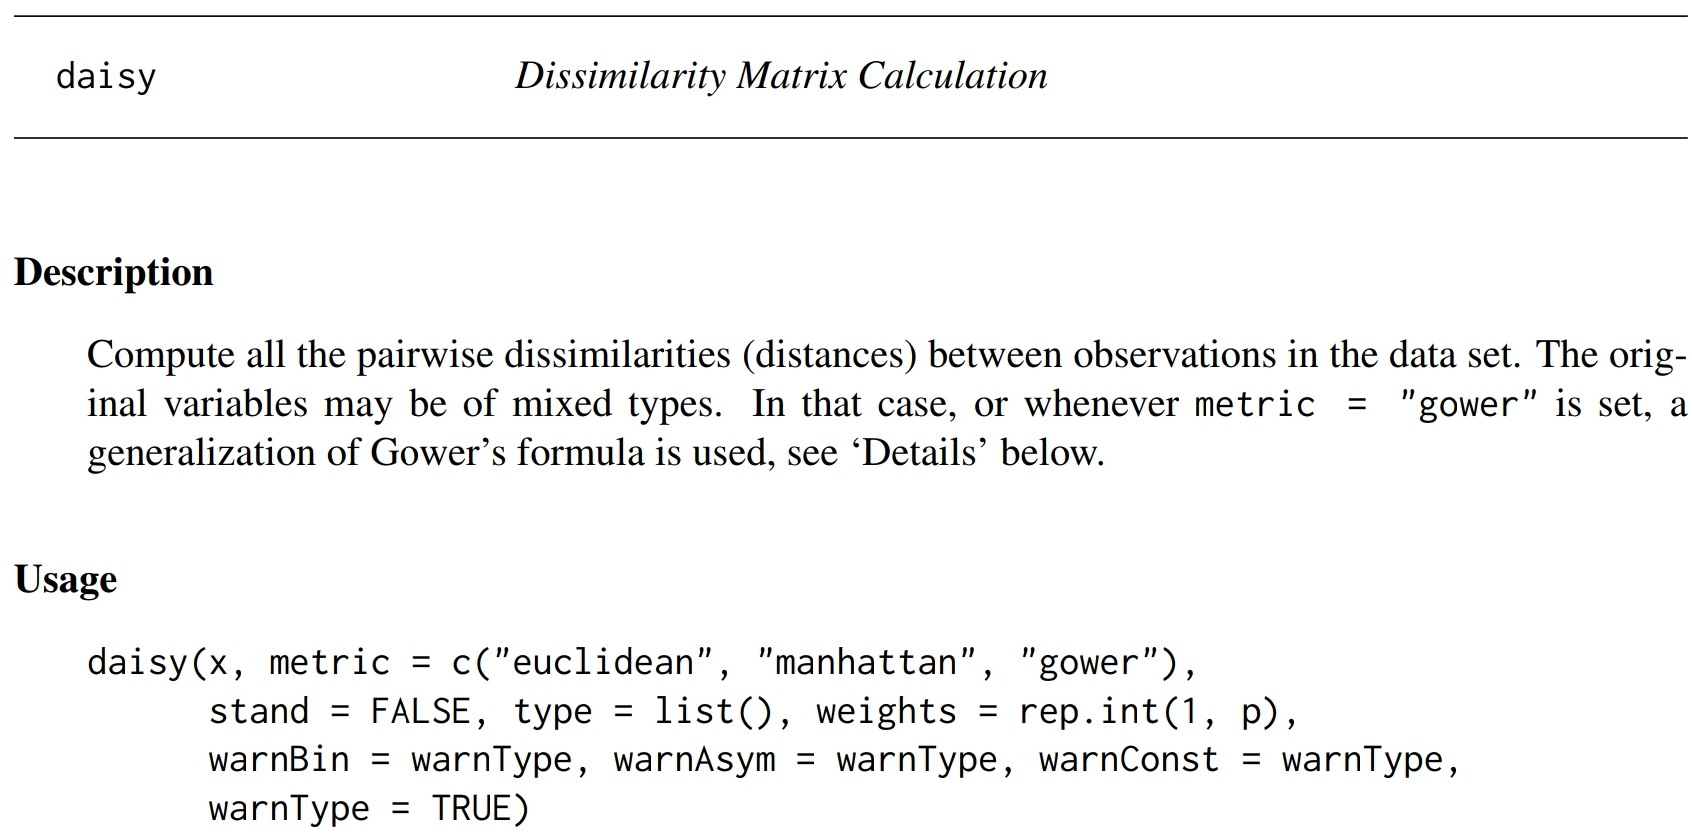
\includegraphics{Daisy.jpg}

\begin{Shaded}
\begin{Highlighting}[]
\KeywordTok{library}\NormalTok{(cluster)}
\NormalTok{(}\KeywordTok{abs}\NormalTok{(}\DecValTok{1-0}\NormalTok{)}\OperatorTok{+}\KeywordTok{abs}\NormalTok{(}\DecValTok{0-1}\NormalTok{)}\OperatorTok{+}\KeywordTok{abs}\NormalTok{(}\DecValTok{0-1}\NormalTok{)}\OperatorTok{+}\DecValTok{1}\OperatorTok{+}\KeywordTok{abs}\NormalTok{(}\DecValTok{1-3}\NormalTok{)}\OperatorTok{/}\DecValTok{2}\OperatorTok{+}\KeywordTok{abs}\NormalTok{(}\DecValTok{3-15}\NormalTok{)}\OperatorTok{/}\DecValTok{17}\OperatorTok{+}\KeywordTok{abs}\NormalTok{(}\DecValTok{150-25}\NormalTok{)}\OperatorTok{/}\DecValTok{180}\OperatorTok{+}\KeywordTok{abs}\NormalTok{(}\DecValTok{50-15}\NormalTok{)}\OperatorTok{/}\DecValTok{50}\NormalTok{)}\OperatorTok{/}\DecValTok{8}
\end{Highlighting}
\end{Shaded}

\begin{verbatim}
## [1] 0.8875408
\end{verbatim}

\begin{Shaded}
\begin{Highlighting}[]
\KeywordTok{daisy}\NormalTok{(data[,}\DecValTok{1}\OperatorTok{:}\DecValTok{8}\NormalTok{],}\DataTypeTok{metric =} \StringTok{"Gower"}\NormalTok{) }
\end{Highlighting}
\end{Shaded}

\begin{verbatim}
## Warning in daisy(data[, 1:8], metric = "Gower"): with mixed variables, metric
## "gower" is used automatically
\end{verbatim}

\begin{verbatim}
## Dissimilarities :
##            1         2         3         4         5         6         7
## 2  0.8875408                                                            
## 3  0.5272467 0.5147059                                                  
## 4  0.3517974 0.5504493 0.5651552                                        
## 5  0.4115605 0.6226307 0.3726307 0.6383578                              
## 6  0.2269199 0.6606209 0.3003268 0.4189951 0.3443627                    
## 7  0.2876225 0.5999183 0.4896242 0.3435866 0.4197712 0.1892974          
## 8  0.4234069 0.4641340 0.6038399 0.2960376 0.4673203 0.5714869 0.4107843
## 9  0.5808824 0.4316585 0.4463644 0.8076797 0.3306781 0.5136846 0.5890931
## 10 0.6094363 0.4531046 0.4678105 0.5570670 0.3812908 0.4119281 0.5865196
## 11 0.3278595 0.7096814 0.5993873 0.6518791 0.3864788 0.4828840 0.5652369
## 12 0.4267565 0.5857843 0.6004902 0.5132761 0.5000817 0.5248366 0.6391340
## 13 0.5196487 0.5248366 0.5395425 0.7464461 0.2919118 0.4524510 0.5278595
## 14 0.2926062 0.5949346 0.6096405 0.3680147 0.5203431 0.3656863 0.5049837
## 15 0.6221814 0.3903595 0.5300654 0.5531454 0.4602124 0.5091503 0.3345588
## 16 0.6935866 0.3575163 0.6222222 0.3417892 0.7301471 0.5107843 0.4353758
## 17 0.7765114 0.1904412 0.5801471 0.4247141 0.6880719 0.5937092 0.5183007
## 18 0.4610294 0.4515114 0.7162173 0.4378268 0.4755310 0.6438317 0.4692402
##            8         9        10        11        12        13        14
## 2                                                                       
## 3                                                                       
## 4                                                                       
## 5                                                                       
## 6                                                                       
## 7                                                                       
## 8                                                                       
## 9  0.6366422                                                            
## 10 0.6639706 0.4256127                                                  
## 11 0.4955474 0.4308007 0.3948121                                        
## 12 0.4216503 0.4194036 0.3812092 0.2636029                              
## 13 0.5754085 0.2181781 0.3643791 0.3445670 0.2331699                    
## 14 0.4558007 0.4396650 0.3609477 0.2838644 0.1591503 0.3784314          
## 15 0.4512255 0.2545343 0.4210784 0.4806781 0.4295752 0.3183007 0.4351307
## 16 0.6378268 0.6494690 0.3488562 0.7436683 0.6050654 0.5882353 0.4598039
## 17 0.4707516 0.6073938 0.3067810 0.7015931 0.5629902 0.5461601 0.5427288
## 18 0.1417892 0.5198529 0.8057598 0.5359477 0.5495507 0.5733252 0.5698121
##           15        16        17
## 2                               
## 3                               
## 4                               
## 5                               
## 6                               
## 7                               
## 8                               
## 9                               
## 10                              
## 11                              
## 12                              
## 13                              
## 14                              
## 15                              
## 16 0.3949346                    
## 17 0.3528595 0.1670752          
## 18 0.5096814 0.7796160 0.6125408
## 
## Metric :  mixed ;  Types = N, N, N, N, O, O, I, I 
## Number of objects : 18
\end{verbatim}

\end{document}
